\documentclass{article}
\usepackage{graphicx}
\usepackage{float}
\title{Applied Statistical Analysis - ProblemSet 3}
\date{2024-11-12}
\author{Eoghan O'Sullivan}

\begin{document}
	\maketitle
	\pagenumbering{gobble}
	%\newpage
	%\pagenumbering{arabic}
	
	\section{Question 1}
	
	For this question, I formulated a research question: "do campaign spending differences affect voteshare?". At the same time, I used R scripting as the statistical method of analysis. The variables were provided in the brief. These were difflog and voteshare, from provided data. The explanatory variable, difflog, is used in the regression analysis as is the outcome variable, voteshare. I produced a regression analysis after determining that the dependent variable follows a normal distribution by showing a bell-shaped curve in a histogram, which I plotted and reviewed. Given it was bell-shaped, I proceeded with a linear regression and below are the results of the analysis.   
	
	\subsection{Part 1}
	\paragraph{Run a regression where the outcome variable is voteshare and the explanatory variable is difflog.}
	For this, I used the lm function in R and created a summary from that object. The two variables were used and the data incumbents\_subset.csv which was read-in and made an object. The results of this regression are in figure 1.
 		\begin{figure}[H]
 			\centering
 				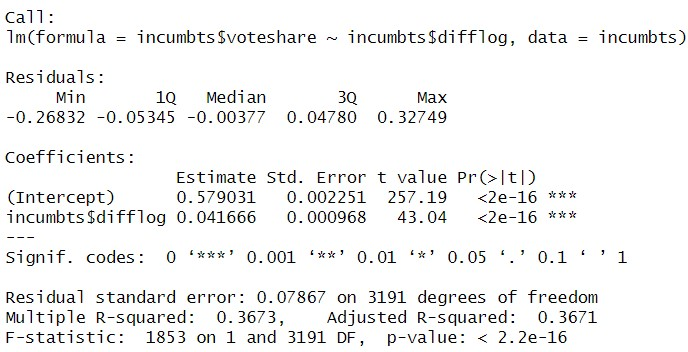
\includegraphics[width=0.9\linewidth]{Question1RegressionAnalysis.jpg}
 				\caption{Regression statistics.}
 				\label{fig:Regression stats}
 		\end{figure}
 	\subsection{Part 2}
 	\paragraph{Make a scatterplot of the two variables and add the regression line.}
 	This task was approached by me using a similar procedure as the last task. I plotted the scatter plot firstly to see if the distribution of data points could be described with a straight line. 
 	When I was confident it was, I fitted a linear model and proceeded to draw the regression line. Below in figure 2 is the resulting graph. To fit the model, I again used the lm function. I created an object called lm\_model. To draw the line I used this object with the abline function for drawing the line and coloured it in red.
 	\begin{figure}[h!]
 	\centering
 		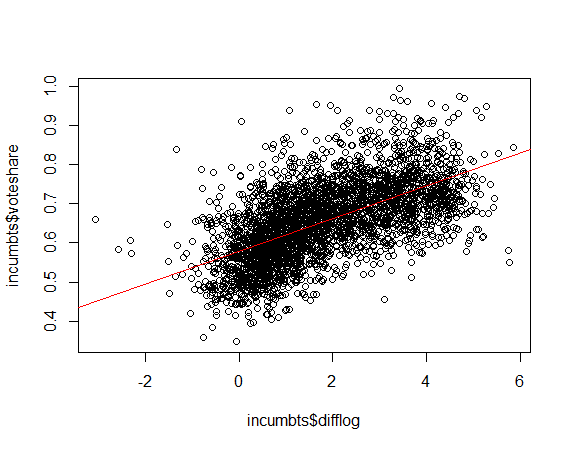
\includegraphics[width=0.9\linewidth]{Question1 - Scatter Plot.png}
 		\caption{Scatter plot with regression line.}
 		\label{fig:Scatter plot with line}
 	\end{figure}
 	 	\subsection{Part 3}
 	\paragraph{Save the residuals of the model in a separate object.}
 	To save the calculated residuals, I made an object called question1\_residuals to store the data for 3193 observations across 20 variables; again with the function lm. 
		\subsection{Part 4}
	\paragraph{Write the prediction equation.}
	I wrote the prediction equation as follows, having calculated the intercept as 
	\begin{equation}
		\beta o
	\end{equation} 
	\paragraph{}and the slope, as 
	\begin{equation}
		\beta x
	\end{equation}The equation is:
	\begin{equation}
		\hat{y} = 0.579 + 0.042 * difflog
		\end{equation}
	\section{Question 2}

	For this question, I formulated a research question: "do campaign spending differences affect presvote?". At the same time, I used R scripting as the statistical method of analysis. The variables were provided in the brief. These were difflog and presvote, from provided data. The explanatory variable, difflog, is used in the regression analysis as is the outcome variable, presvote. I produced a regression analysis and below are the results of the analysis.   
\subsection{Part 1}
\paragraph{Run a regression where the outcome variable is presvote and the explanatory variable is difflog.}
The results of this regression are in figure 3.
\begin{figure}[H]
	\centering
	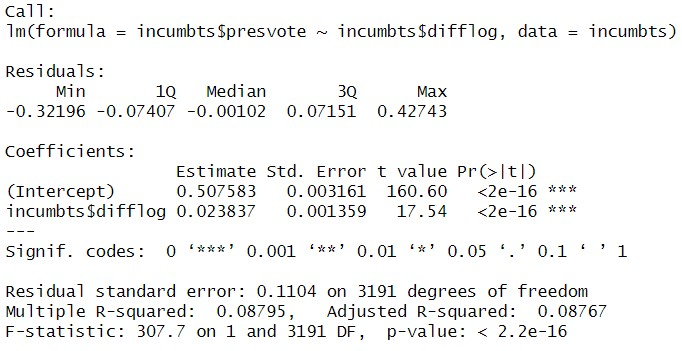
\includegraphics[width=0.9\linewidth]{Question2RegressionAnalysis.jpg}
	\caption{Regression statistics.}
	\label{fig:Regression statistics}
\end{figure}
\subsection{Part 2}
\paragraph{Make a scatterplot of the two variables and add the regression line.}
I was confident the scatter plot showed a a straight line and I then fitted a linear model and proceeded to draw the regression line. Below in figure 4 is the resulting graph. To fit the model, I again used the lm function. This time, I again created an object called lm\_model. To draw the line I used this object with the abline function for drawing the line and coloured it in red.
\begin{figure}[h!]
	\centering
	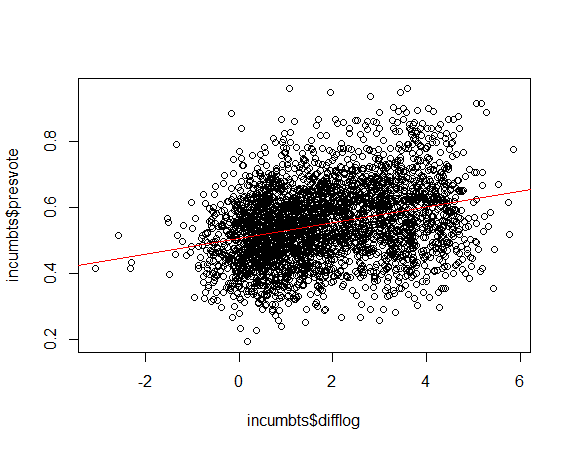
\includegraphics[width=0.9\linewidth]{Question2 - Scatter Plot with regression line.png}
	\caption{Scatter plot with regression line.}
	\label{fig:Scatter plot with regression line}
\end{figure}
\subsection{Part 3}
\paragraph{Save the residuals of the model in a separate object.}
To save the calculated residuals, I made an object called question2\_residuals to store the data for 3193 observations across 20 variables; again with the function lm. 
\subsection{Part 4}
\paragraph{Write the prediction equation.}
I wrote the prediction equation as follows, having calculated the intercept as 
\begin{equation}
	\beta o
\end{equation} 
\paragraph{}and the slope, as 
\begin{equation}
	\beta x
\end{equation}The equation is:
\begin{equation}
	\hat{y} = 0.508 + 0.024 * difflog
\end{equation}
\section{Question 3}

For this question, I formulated a research question: "how does the incumbent President's party vote share affect his/her electoral success?". The variables were provided in the brief. These were presvote and voteshare, from provided data. The explanatory variable, presvote, is used in the regression analysis as is the outcome variable, voteshare. I produced a regression analysis after determining that the dependent variable follows a normal distribution by showing a bell-shaped curve in a histogram, which I plotted and reviewed. Given it was bell-shaped, I proceeded with a linear regression and below are the results of the analysis.   
\subsection{Part 1}
\paragraph{Run a regression where the outcome variable is voteshare and the explanatory variable is presvote.}
The results of this regression are in figure 5.
\begin{figure}[H]
	\centering
	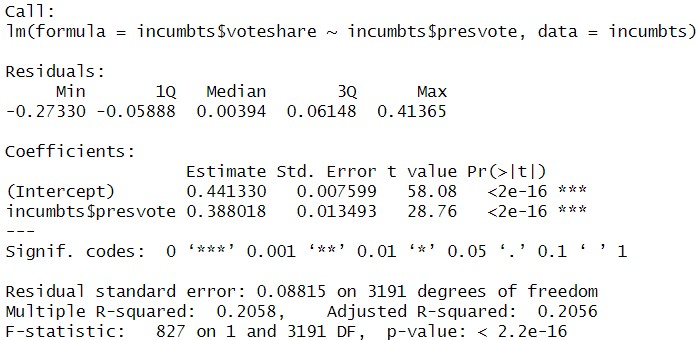
\includegraphics[width=0.9\linewidth]{Question3RegressionAnalysis.jpg}
	\caption{Regression statistics.}
	\label{fig:Regression statistics}
\end{figure}
\subsection{Part 2}
\paragraph{Make a scatterplot of the two variables and add the regression line.}
I was confident the scatter plot showed a straight line and I then fitted a linear model and proceeded to draw the regression line. Overleaf in figure 6 is the resulting graph. To fit the model, I again used the lm function. I created an object called lm\_model. To draw the line I used this object with the abline function for drawing the line and coloured it in red.
\begin{figure}[H]
	\centering
	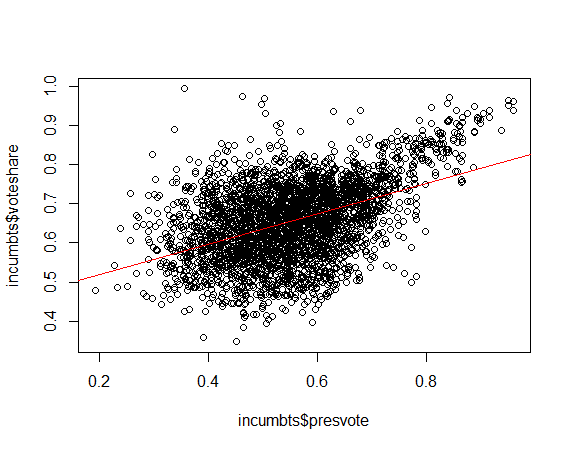
\includegraphics[width=0.9\linewidth]{Question3 - Scatter Plot with regression line.png}
	\caption{Scatter plot with regression line.}
	\label{fig:Scatter plot with regression line}
\end{figure}
%\subsection{Part 3}
%\paragraph{Save the residuals of the model in a separate object.}
%To save the calculated residuals, I made an object called question2\_residuals to store the data for 3193 observations across 20 variables; again with the function lm. 
\subsection{Part 3}
\paragraph{Write the prediction equation.}
I wrote the prediction equation as follows, having calculated the intercept as 
\begin{equation}
	\beta o
\end{equation} 
\paragraph{}and the slope, as 
\begin{equation}
	\beta x
\end{equation}The equation is:
\begin{equation}
	\hat{y} = 0.441 + 0.388 * presvote
\end{equation}
	\section{Question 4}
This question I approached by using previously calculated residuals.
\subsection{Part 1}
\paragraph{Run a regression where the outcome variable is the residuals from Question 1 and the explanatory variable is the residuals from Question 2.}
The results of this regression analysis are below in figure 7. 
\begin{figure}[h!]
\centering
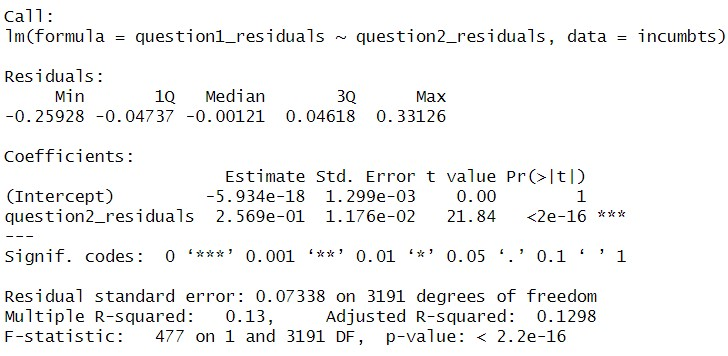
\includegraphics[width=0.9\linewidth]{Question4RegressionAnalysis.jpg}
\caption{Regression statistics.}
\label{fig:Regression statistics}
\end{figure}
\subsection{Part 2}
\paragraph{Make a scatterplot of the two residuals and add the regression line.}
I approached this by using the lm function in R and wrote as arguments the residuals from questions 1 and 2 and the data itself. The graph in figure 8 refers.
\begin{figure}[h!]
	\centering
	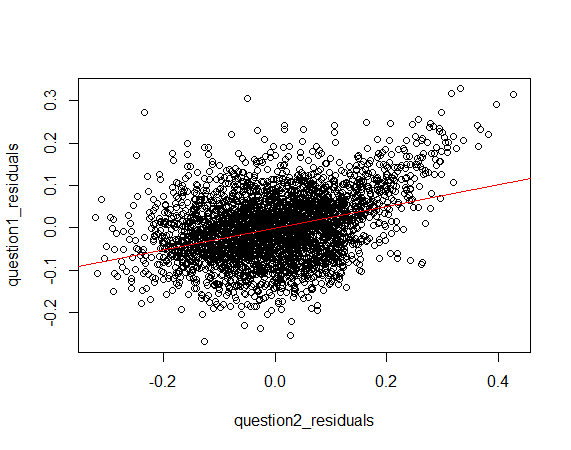
\includegraphics[width=0.9\linewidth]{Question 4 - Scatter Plot with regression line.png}
	\caption{Scatter plot with regression line.}
	\label{fig:Scatter plot with regression line}
\end{figure}



	\section{Question 5}

For this question, I formulated a research question: "Is the incumbent's voteshare affected by both the president's popularity and spending differences?". At the same time, I used R scripting as the statistical method of analysis. The variables were provided in the brief. These were difflog, voteshare and presvote from provided data. The explanatory variables, presvote and difflog, are used in the regression analysis as is the outcome variable, voteshare. I reviewed assumptions and I proceeded with a multivariate regression and below are the results of the analysis.   
\subsection{Part 1}
\paragraph{Run a regression where the outcome variable is the incumbent's voteshare and the explanatory variables are difflog and presvote.}
For this part, I used the lm function in R and created a summary from that object.  The results of this regression are in figure 9.
\begin{figure}[H]
	\centering
	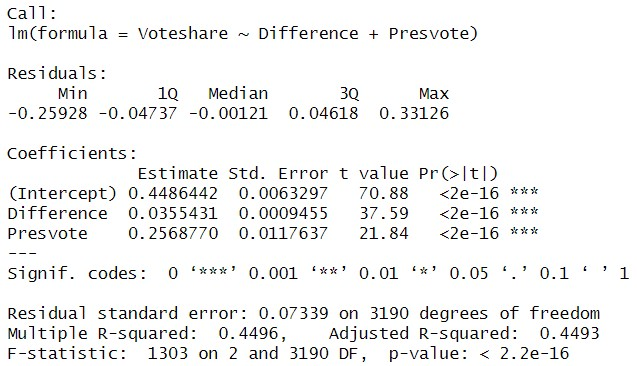
\includegraphics[width=0.9\linewidth]{Question5RegressionAnalysis.jpg}
	\caption{Regression statistics.}
	\label{fig:Regression stats}
\end{figure}
\subsection{Part 2}
\paragraph{Write the prediction equation.}
I wrote the prediction equation as 0.449 + 0.257 * difflog + 0.036 * presvote
\end{document}